\clearpage
\section{Coursework 2 (Part 1): \\ Smarter Robot Controllers}

In the second coursework you are required to develop
sophisticated robot controllers which adopt a more systematic approach to
exploring a maze and that learn. In the first part of this coursework we will
initially build a controller that systematically searches a dense maze (one
that does not contain loops). In such mazes the
empty squares form a network (or tree) of corridors one square wide. 
There are additional exercises at the end of Part 1 whereby we extend
this controller
so that it is able to deal with loopy mazes\footnote{Mathematically this
means extending our robot from one that explores {\em trees} to one that
explores {\em graphs}.}.\\

\noindent
For the second part of the coursework you will be asked to
create a robot controller that learns from its previous runs. This means that
the more a robot explores (the same maze), the quicker it gets at finding the
target.\\

\noindent
To complete these exercises you will need to be familiar with the use of arrays in
Java. You will find plenty of examples dedicated to the use of arrays in the lecture
notes; you will also find good coverage of arrays in the recommended
course textbooks.\\

\noindent
The control programs which you will write will be more complicated
than those from the earlier chapters. As such, you will find that they are much
more manageable if you split them up by writing components as separate
methods. As a rough guide you should aim to keep each individual method
below 30 lines in length. Similarly, you will almost certainly find it
worth your while packaging useful bits of code from earlier questions (e.g.
choosing a random direction etc.) into methods for later re-use.\\

\noindent
In these exercises you are also required to develop your own Java class(es)
from scratch. This is an important part of code design and you will find that
you can reuse some of these classes in the solutions to the questions in
Chapter 9. It is important not to shy away from the inclusion of your own
classes. Apart from anything else, it will ensure that you gain a better
grade when your solutions are marked. \\

\noindent
This coursework, like the first, is split into two parts. You will find that
you are guided through the first part of the coursework but not the second.
The reason for this is that Part 2 is intended to be tricky and challenge the best students. 
Even if you do not complete
these every exercises, you may find that you pick up marks for partial 
solutions (or even non-working solutions), so it is worth having a go at these 
questions if you have time.\\

\noindent
All your solutions must
be complete by \deadlinetwo. You should remind
yourself of the rules for coursework by taking a quick look at the first page
of Chapter 6.


\subsection{Exercise 1}

$\diamondsuit$
An entirely new {\tt Explorer} robot controller is going to be built; this
should be done
in a file called {\tt Explorer.java}. This new controller should ensure
that the robot meets the following specification:

\begin{itemize}

\item
The robot should never reverse direction, except at dead ends.

\item
At corners it should turn left or right so as to avoid collisions.

\item
At junctions it should, if possible, turn so as to move into a square that
it has not previously been explored, choosing randomly if there are more than one.
If this is not possible it should randomly choose a direction that doesn't
cause a collision.

\item
Similar behaviour to junctions should be exhibited at crossroads:
the robot should select an unexplored exit if possible, selecting
randomly between the exits if more than one is possible. If there
are no unexplored exits then the robot should randomly choose a
direction that doesn't cause a collision.

\end{itemize}

\noindent As the specification suggests, there are four cases to
consider, the direction chosen if the robot is: at a dead end; travelling down
a corridor; at a junction; and at a crossroads.\\

\noindent
We can tell which of these cases we need to consider at any one time
by developing a method called {\tt nonwallExits}, running it and
observing the result. \\

\noindent
{\bf Design step 1:} Add a method {\tt nonwallExits} to your {\tt
Explorer.java} file which returns
the number of non-{\tt WALL} squares (exits) adjacent to the square currently
occupied by the robot. You will need to use the {\tt robot.look} method
and check all four directions. As a guide, your solution should not be more
than ten lines of Java code. \\

\noindent
You should check that you have not made any syntax errors by compiling your
solution. You will need to make sure that you have incorporated
the {\tt import} statement at the beginning of the file, you will also
need an {\tt Explorer} class which includes an empty {\tt controlRobot}
method as well as the new {\tt nonwallExits} method, e.g. \\

\begin{verbatim}
  import uk.ac...

  public class Explorer {
    public void controlRobot(IRobot robot) {}

    private int nonwallExits (IRobot robot) {  // Your new method
      ...
    }
  }
\end{verbatim}

\noindent
After some debugging you will find that the compiler no longer
complains. Of course you cannot run this
program yet as the controller code does not do anything. \\

\noindent
If the {\tt nonwallExits} method returns a result that is less
than two, then the robot is at a dead end; if the robot is
travelling down a corridor, then the number of non-wall exits
will be exactly two; if the number of non-wall exits is three
then the controller has detected that the robot is at a junction;
and finally, if the number of non-wall exits
is four then the robot is at a crossroads. See Figure~\ref{explorer} for details. \\

\noindent
A sensible way to proceed with the development of the explorer
robot is to design the method {\tt controlRobot} so that it
detects which of these four cases it is dealing with. If the robot
is travelling along a corridor, then the control method can pass
control to a subsidiary method which determines what to do in
this case. Likewise, the
dead-end, junction and crossroad cases can be developed in the same way. \\

\noindent
{\bf Design step 2:} Modify the {\tt controlRobot} method so that
it records the result of calling the {\tt nonwallExits} method. Store
the result in a variable called {\tt exits}. \\

\noindent 
{\bf Design step 3:} Now extend the  {\tt controlRobot}
method so that it passes control to four sensibly named subsidiary
methods depending on the value of the {\tt exits} variable.\\

\noindent
You will probably want these four subsidiary methods to return
direction values to your controller. Your controller therefore,
will need to introduce a variable {\tt direction} and assign the
result of calling the subsidiary method to that, e.g. \\

{\tt direction = deadEnd(robot);}\\

\noindent
The {\tt controlRobot} method will need to
execute the command {\tt robot.face(direction)} before it terminates. \\

\noindent
You can compile your changes to check for any syntax errors. You
will need to include empty definitions of your subsidiary methods
if the compilation is to succeed. The next task is to write the
four subsidiary methods. We will look at each of these in turn. \\

\begin{figure}[t]
\centering
\includegraphics[width=3in]{explorer.eps}
\caption{There is a clear relationship between the number of
non-wall exits and the situation which the {\tt Explorer} robot
finds itself in; this is demonstrated in the above figure.
\label{explorer}}
\end{figure}

\noindent {\bf Design step 4:} {\it Dead ends} -- What
should the robot do if it is at a dead end? Well, you are nearly
right. It should turn round and head back in the direction it
came from in all but one case -- when it is at the start. Write
the first of the four subsidiary methods to deal with the case
when the robot is at a dead end. This will not require too much
code as all you need to do is get the robot to find the one and
only non-wall route.\\

\noindent
{\bf Design step 5:} {\it Corridors} -- If the robot is travelling down a
corridor, or is at a corner, then control should be
passed to the corridor subsidiary method. This method will ensure that
when in a corridor the robot will not crash into walls (of course) and
that it will not reverse direction and go back on itself, since it only
does this at dead ends. Write this second subsidiary method; again it
should not be longer than about ten lines of code. \\

\noindent 
{\bf Design step 6:} {\it Junctions} -- At a junction
the robot controller should select a {\tt PASSAGE} exit if one
exists. This ensures that the robot explores new parts of the
maze in preference to exploring parts of the maze which it has
already visited. If there are no passage exits the robot should
choose randomly between all non-wall exits. \\

\noindent 
{\bf Design step 7:} {\it Crossroads} -- The final
subsidiary method is the control code for crossroads. This should
exhibit similar behaviour to that of the junction controlling
method: selecting an unexplored exit if possible, selecting
randomly between these unexplored exits if more than one is
possible and, if there are no unexplored exits, randomly
selecting a direction that doesn't cause a collision. \\

\noindent
You might find it useful to define an additional {\tt
passageExits} method. This will be similar to your {\tt
nonwallExits} method but instead it will return the number of
passage exits in relation to the robot position.\\

\noindent
Implementing the junction and crossroad control methods then
becomes simple. If there are one or more {\tt PASSAGE} exits then
the controller should choose one of the passages randomly; if
there are no {\tt PASSAGE} exits then the controller should choose
randomly between all non-wall exits. \\

\noindent
When you have completed the code you should compile it to remove all the
errors. When you have finished this you should have a new {\tt Explorer.class}
file which can be loaded into the robot-maze environment.
Test your robot controller carefully to ensure that it meets the specification.\\

%\noindent
%When you are satisfied that it works correctly, be sure to save
%the {\tt Explorer.java} file in {\tt Ex1.java} otherwise you will
%receive no marks for this exercise.

\subsubsection{Storing data}

$\diamondsuit$
You will notice that the explorer robot is very good when it comes to searching
areas of the maze which it has not been to before. However, when part of the
maze is thoroughly searched it is unfortunate that the robot goes into {\it random}
mode. It would be better if the robot were able to follow its path back to the
point at which it chose between one unexplored path or another. This
would enable the robot to backtrack to a previously encountered junction and
follow any previously unexplored exits. \\

\noindent
This is the behaviour of the robot controller which will be built in the
next two parts of this chapter. In order to do this,
the controller {\tt Explorer.java} will be modified so that, whenever
a junction is encountered which the robot has not previously encountered in its
current run, its location and the heading the robot arrived from are
recorded. This information will then be used in the implementation of a
{\it backtracking}~routine. \\

\noindent {\bf Design step 1:} You can easily detect whether a
junction or crossroads has already been visited during a robot run
by counting the number of adjacent {\tt BEENBEFORE} squares. If
there are more than one, the robot Explorer must have
visited the junction or crossroads at least once before. \\

\noindent Write a method called {\tt beenbeforeExits} that is
similar to the method {\tt passageExits} which you defined 
previously. This method will return the number of {\tt
BEENBEFORE} squares adjacent to the robot. \\

\noindent {\bf Design step 2:} The recording of junction and
crossroad information\footnote{From here on in the text I will
refer to junctions/crossroads simply as junctions. The smart
ones amongst you will have realised that there is in fact no
difference in the treatment of the two.} will be implemented in a
separate class which should be named {\tt RobotData}. This new
class can be included as part of the {\tt Explorer.java} file and
should contain local state
information for each junction the robot encounters. \\

\noindent When a junction is reached your robot should store the
{\it x}- and {\it y}-coordinates (to uniquely identify it) and the
{\it absolute} direction which the robot arrived from when it first encountered
this junction. This information can be stored in three arrays, i.e., 

\begin{verbatim}
 private static int maxJunctions = 10000; // Max number likely to occur
 private static int junctionCounter; // No. of junctions stored  
 private int[] juncX;            // X-coordinates of the junctions
 private int[] juncY;            // Y-coordinates of the junctions
 private int[] arrived;          // Heading the robot first arrived from
\end{verbatim}

\noindent An implementation which looked like this would be
quite adequate. However, you might decide that an array of {\tt
JunctionRecorder} objects or
something similar would be a better implementation (and indeed it would).\\

\noindent
The coordinates and arrived-from direction for the {\em i}-th
freshly unencountered junction will be stored in the {\em i}-th
elements of the arrays. You can do this by using an integer
variable ({\tt junctionCounter}, say) to count the number of
junctions for which information has been recorded.\\

\noindent
On the first pass of a new run {\tt junctionCounter} should be
set to 0. This can be done by observing the {\tt robot.getRuns()}
method which allows the control program to detect when it is
computing the first run through a maze (see Section 4.2.9). This
value alone is not enough as it will remain 0 throughout the
robot's first run through the maze. What you need to do is
include a counter which counts the number of times the controller
code is polled. A combination of these values will allow you to
detect the first move in a first run through a
new maze. \\

\noindent
The code for this might look something like: \\

\begin{verbatim}
  public class Explorer {
    private int pollRun = 0;     // Incremented after each pass
    private RobotData robotData; // Data store for junctions
    ...

    public void controlRobot(IRobot robot) {
      ...
      // On the first move of the first run of a new maze
      if ((robot.getRuns() == 0) && (pollRun == 0))
         robotData = new RobotData(); //reset the data store
      ...
      pollRun++; // Increment pollRun so that the data is not
                 // reset each time the robot moves
    }
  ...
\end{verbatim}

\noindent where the constructor code for {\tt RobotData} does
something sensible -- such as setting {\tt junctionCounter} to
zero, for example. \\

\noindent
Complete and insert this code into the {\tt Explorer.java} file. \\

\noindent
This is a tricky part of the Explorer code as you are having to
manage the introduction of your new {\tt RobotData} class as well
as interfacing with the maze-environment itself. In order to pull
this off you need to add the method

\begin{verbatim}
   public void reset() { 
      robotData.resetJunctionCounter(); 
   }
\end{verbatim}

\noindent to the {\tt Explorer} class in which you are developing
your controller code, and then add to your {\tt RobotData} class
the method \\

\begin{verbatim}
   public void resetJunctionCounter() {
      junctionCounter = 0; 
   }
\end{verbatim}

\noindent What this does is ensure that when you press the {\bf
Reset} button in the maze-environment your {\tt junctionCounter}
variable will be reset\footnote{You must follow these
instructions otherwise you will get into 
trouble in the next exercise.}. \\

\noindent {\bf Design step 3:} Now modify the {\tt controlRobot}
method so that each time the robot arrives at a previously
unencountered junction the coordinates and the direction the
robot arrived from are stored in the {\tt junctionCounter}
elements of each
array. Remember to increase the {\tt junctionCounter} by 1. \\

\noindent
A nice way to carry out this recording of junction information is to extend
the {\tt RobotData} class so that
it includes a {\tt recordJunction} method. This method might take three
parameters: the {\em x}-coordinate of the junction (which you can access
by making a call to {\tt robot.getLocation().x}); the {\em y}-coordinate of
the junction (which you can access by making a call to
{\tt robot.getLocation().y});
and the robot heading (which you can access by calling
{\tt robot.getHeading()}).\\

\noindent
{\bf Design step 4:}
When you have completed these modifications, test that the information
recorded is
correct by printing it out on the screen (using a {\tt printJunction()} method)
and comparing it with the simulation display. \\

\noindent
If you are in any doubt as to what the result of this exercise is
then consider the following scenario: In Figure~\ref{helpful} we
see that the robot has passed through three junctions. In this
case one would expect the robot to record (and print using
the {\tt printJunction()} method) the following information:

\begin{figure}[t]
\centering
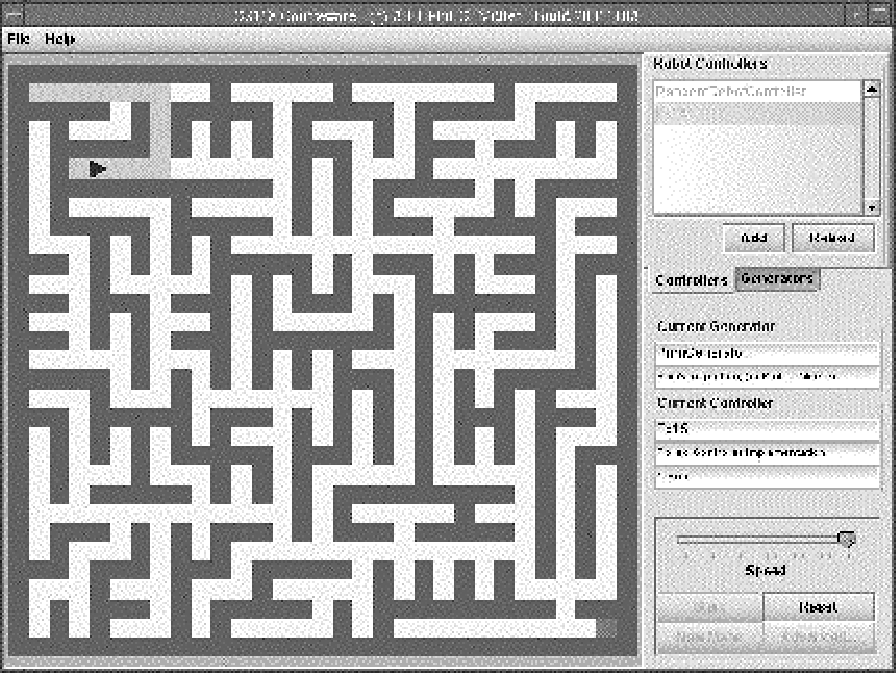
\includegraphics[width=4.5in]{helpful.pdf}
\caption{The robot has passed through three junctions. The information
which is stored in your new {\tt RobotData} class includes the x- and
y-coordinates of these junctions as well as the heading of the robot 
as it arrived at these junctions.
\label{helpful}}
\end{figure}

\begin{verbatim}
    Junction 1 (x=5,y=1) heading EAST
    Junction 2 (x=7,y=1) heading EAST
    Junction 3 (x=7,y=5) heading SOUTH
\end{verbatim}

\noindent
In order to verify that the output of your program is correct in
relation to the movement of the robot, you will have to run your
robot very slowly. Reset your robot every now and then and trace
through the route of the robot and the output you get from {\tt
printJunction()}, just to make sure that the information which you
record is correct.

%\noindent
%Save your answer to this exercise as {\tt Ex20.java}.
%Remember, no file, no marks.


\subsubsection{Using stored data}

$\diamondsuit$
Modify the {\bf Explorer} robot so that it uses the information it records to
perform a systematic search for the target. The specification for the new
robot is as follows:

\begin{itemize}

\item
Initially the robot will {\em explore}.

\item
When the robot is {\em explore}-ing it behaves like the original
{\tt Explorer} robot except that when it reaches a dead end or a junction
that it has already encountered in the same run, it should reverse direction
and {\em backtrack}.

\item
If the robot encounters a junction with unexplored exits while
{\em backtrack}-ing it should choose one of these exits randomly
and {\em explore} down it.

\item
If the robot encounters a junction with no unexplored exits while
{\em backtrack}-ing it should {\em backtrack} in the direction from which
it came when it first reached the junction. This behaviour is termed
`backtracking through' a junction.

\end{itemize}

\noindent
All this may sound complicated but it is not. What the robot controller is
really doing here is switching between two states, the {\em exploring}
state and the {\em backtracking} state. This switch can be implemented as
a state variable of the {\tt Explorer} class,

\begin{verbatim}
  private int explorerMode;  // 1 = explore, 0 = backtrack
\end{verbatim}

\noindent
for example. \\

\noindent
{\bf Design step 1:}
Add the {\tt explorerMode} variable to your code and set it in your
control code so that when the robot begins a new run the mode is
appropriately initialised\footnote{The robot should start off in explorer mode.
You can ensure that this is the case by adding an appropriate line of code just
after your call to {\tt new RobotData();}. To ensure that you get the same
effect when the {\bf Reset} button is pressed, you should also add this line
of code to the {\tt reset()} method which you introduced in the previous
exercise.}. \\

\noindent
We now need to implement two controllers,
{\tt exploreControl} and
{\tt backtrackControl}. The robot will be able to
switch between these states depending on the
situation. \\

\noindent
{\bf Design step 2:}
The method {\tt exploreControl} is pretty much the same code as you
used previously. You should define a new method called
{\tt exploreControl} in your {\tt Explorer} class.
When you have done this, cut the explorer code out of {\tt controlRobot}
and paste it into {\tt exploreControl}. You will find that the
{\tt controlRobot} method then contains just the basic
control code which detects if it is a new run etc. and of course, a call
to the new {\tt exploreControl} method.\\

\noindent
To complete the {\tt exploreControl} method you also need to add
the code which sets the {\tt explorerMode} switch to zero when you reach
a dead end. \\

\noindent
{\bf Design step 3:}
The {\tt backtrackControl} method will require a call to a
{\tt searchJunction} method (which should also be defined as part of your
{\tt RobotData} class) which is used to search the {\tt RobotData}
for a junction which has already been encountered. This will return the
direction that the robot was travelling when it originally arrived at the
junction. \\

\noindent
Write the method {\tt searchJunction} which, when given the {\it x}- and
{\it y}-coordinates of the robot, will return the robot's heading when it
first encountered this particular junction.  What will this method
return if it is called when the robot is at a junction which it has not
previously encountered? \\

\noindent
{\bf Design step 4:} Your backtracking control method can now be
written. Start by introducing a new method {\tt backtrackControl},
below your {\tt exploreControl} method, in the {\tt Explorer} class.
Design your backtrack
control method so that it calculates the number of non-wall exits
in relation to the robot's position -- this is a similar framework to
the {\tt exploreControl} function.\\

\noindent
If the number of non-wall exits is greater than two, then the
robot is at a junction or crossroad. The backtracking control method
then needs to detect if there are any {\tt passageExits} at this junction:
if there are, then the robot must switch back into explorer mode
and then proceed down one of these unexplored paths (choosing
randomly between them if there are more than one); if there are
no passage exits then the robot must exit the junction the
opposite way to which it FIRST entered the junction. You can use
the {\tt searchJunction} method to determine the initial heading
of the robot when it first entered the junction -- the controller
should calculate the reverse of this and head the robot in that
direction\footnote{See Section 5.2.4.}.\\

\noindent
If the number of non-wall exits is two or less, then the backtracking
method should use the existing methods which select a direction at a
corridor and select a direction at a dead end respectively. \\

\noindent
{\bf Design step 5:} There is one further design step which you need to make
and that is to consider what the controller should do when the robot is
at the very first square. \\

\noindent
If you have any doubts as to what all this means then talk to your
seminar tutor. Time will be set aside in the seminars to discuss these set of
problems. \\

\noindent Save your answer to this exercise as {\tt Ex1.java}. No
file; no marks.

\subsubsection{Worst case analysis}

$\diamondsuit$
Will the robot {\bf Explorer} always find the target using this strategy? Can you place
a limit on the length of time (or maximum number of steps) it will take {\bf Explorer} to find the target?
Explain your answers.


\subsection{Exercise 2}

In a `real life' situation it may be highly desirable to minimise the amount
of data storage required by the control program. \\

\noindent
$\diamondsuit$ Re-implement your robot controller so that the systematic search strategy of
the {\bf Explorer} robot does not require the \emph{location} of
each junction to be recorded. \\

\noindent
Save your solution to {\tt Ex2.java}.


\subsection{Depth-first search in path finding}

Throughout this chapter you have been working on the solution to a
well-documented {\it search problem}. These sorts of problems are ubiquitous,
cropping up everywhere in Artificial Intelligence and in other areas of
Computer Science.\\

\noindent
Imagine taking our maze and picking it up from the robot's start position.
You can lift the maze up so that it hangs like a mobile; it will look
like an inverted tree (see Figure~\ref{mobile}). You will notice that each path through
the maze becomes a branch in the tree, terminating at a leaf when a
dead end is reached. The target will appear on one of the branches in the
tree.\\

\begin{figure}
\centering
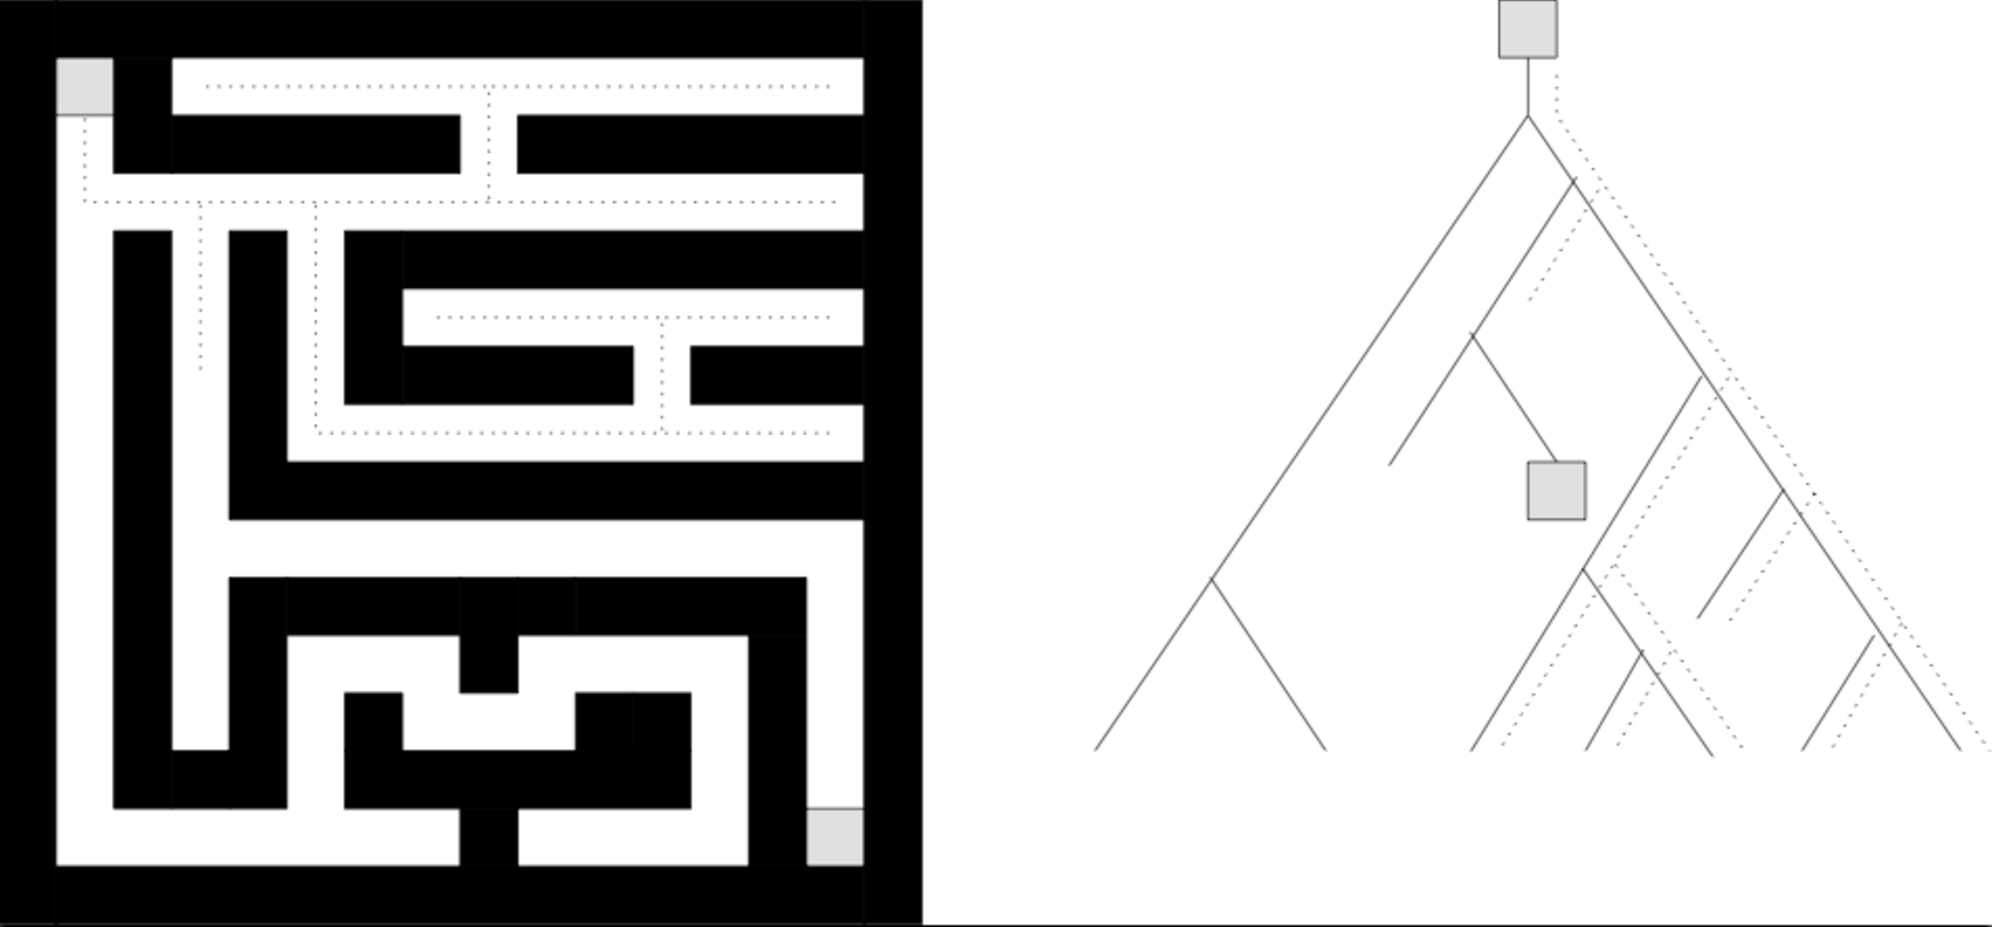
\includegraphics[width=4in]{mobile.pdf}
\caption{Representing the maze as a search tree \label{mobile}}
\end{figure}

\noindent
Consider what happens when the explorer robot searches the maze. First it
will choose one path of the maze. The robot will thoroughly search the part
of the maze which this path leads to; any unexplored exits will be
searched until, if the target is not detected, the robot backtracks to the
junction at which the initial choice was made.\\

\noindent
This procedure is analogous to searching one part of the maze-tree. Given
that one initial path is as likely to be as good as any other, searching
the tree requires picking an alternative at every node in the tree and
working forward from that alternative. Other alternatives at the same
level are ignored as long as there is a hope of reaching the
target using the original choice. This search strategy is known as
a {\it depth-first search}.\\

\noindent
The search proceeds to the bottom of the tree if the target is not found;
it then backs up to the nearest ancestor node with an unexplored alternative.
If this path does not work out then the procedure will move still further
back up the tree seeking another viable decision point to move forward from.
This process continues until the target is reached or all possible paths in
the tree are exhausted. \\

\noindent
There are many other search techniques which are used to solve this and
similar problems in Computer Science. Some of these search techniques will
be more efficient, others will be more suited to finding the {\it shortest
path}. Special-case procedures also exist which are appropriate when
facing an adversary. These procedures use {\it game trees} and are common
in computer programs that play board games such as chess for example.

\subsection{Exercise 3}

\subsubsection{Single loops}

Currently our {\bf Explorer} robot uses a depth-first search. This is all very 
well as long as our maze is non-loopy -- as soon as a loop is introduced the
exploring algorithm breaks\footnote{You can test this out for yourself.}.\\
 
\noindent
$\diamondsuit$ Modify your {\bf Explorer} robot so that it is able to navigate mazes with 
single loops. Some of you may find it easier to work from your Exercise 1 answer,
others may find it easier to extend from Exercise 2. \\

\subsubsection{Multiple loops}

$\diamondsuit$
Extend your answer so that your robot can navigate
mazes with multiple loops. \\

\noindent
Save your solution to {\tt Ex3.java}. \\

\noindent
Solving loopy mazes has been the subject of much research\footnote{From
longer ago than you might think -- from the ancient Minoans in Crete in
about 2000~BC, to our very own upper-class and bored Royalty, with nothing better
to do than frolic around in daft clothes and in houses large enough
to host a maze in their outside privy.}
and as you might expect, someone has already contemplated the problem of
navigating around a maze with multiple loops. Indeed a nice solution to
this problem was originally published in {\em Recreations Mathematique}
(Volume 1, 1882) by M. Tr\'{e}maux. 

\subsection{Summing up}

You have now reached the end of the first set of exercises of Coursework 2.
Getting this far in the exercises will probably be enough to ensure that you
get a pass grade for the practical component of the
Programming for Computer Scientists course (providing your
code works, has comments, looks nice etc.)
Before you go off and celebrate, you must ensure that you 
submit a copy of the files {\tt Ex1.java}, {\tt Ex2.java}, and {\tt Ex3.java}.  \\

\noindent
Make sure that you change the class name at the top of each file from 
{\tt Explorer} to {\tt Ex*} such that they compile correctly. Then submit your
solutions through Tabula.
